\chapter{Our Approach}
\label{sec:our-approach}

\section{System Architecture}

- Basically, two kinds of users and administrators that interact with the system.
- No typical system: Both users want to interact as less as possible manually with the system 

IMAGE: C4-System overview image

A redbackup system consists of on management, multiple interconnected nodes as well as clients.
TODO: explain roles and components in more details...

Redbackup specifies a high-level protocol that is used for internal communication.

reference specification for more details

IMAGE: C4-designed system

% Brief introdcution of all actors, components and messages
% The specification is complicated because it is the result of long discussions and a clarification process (See https://project.redbackup.org/browse/REDPRO-98)
% See Describing architectures in https://wiki.hsr.ch/FarhadMehta/files/Writing_Scientific_Papers.pdf
% Describe everything concise and with exact definitions.
% Use schemes and flowcharts

\subsection{Replication}
% Planned and unplanned leaving of nodes
% Management down

- briefly discuss sequence diagram
- discuss what happens if the management is down

\subsection{Partitioning \& Scaling}
% Communication

- storage and node are typically bundeled
- management on a spearate host
- scalability: run multiple nodes
 - if a node has overload: client can use another node
 - eventual consistency
- 


\subsection{Failure Detection}
% Corrupted Storage
% Management/Node down
% Network Availability Problems

- if storage detects corruption:
    - perform periodic checks
    - node can notify management or ask other nodes if they have a "safe" copy
- more from specification?
- TODO: more things from fault tolerance book?

\section{Fundamental Design Decisions}

We used the morphological box technique to explore different possible solutions (See Table \ref{tbl:morphological-box})

The chosen option should be as simple as possible for the prototype developed in the study project but extensible for further adaption.

The following paragraphs reason the selected entry in each dimension.

\paragraph{Redundancy} 
We originally planned to support \emph{client m-replication}, which means that the client defines a custom degree of redundancy from 1 to the number of nodes. This, however, is a complex mechanism that requires sophisticated algorithms to work correctly and efficiently. For the prototype, we chose the more straightforward to implement option system \emph{n-replication}, where the degree of redundancy for the whole system is equal to the number of nodes in it. Changing this option in the future is hard because it requires fundamental changes in the replication process and the communication protocols.

\paragraph{Storage unit}
The idea of \emph{chunks} come from Borg Backup. Files are partitioned into chunks using a rolling hash which allows deduplication as well as space efficient backups for large files \cite{borg-data-structures}. These are desired properties in a backup system to minimise network and disk usage.

\emph{Encrypting chunks} means that deduplication of the same file coming from different users is not possible anymore but is a necessity for privacy. Encryption is not trivial and requires a user concept that is out of scope of the prototype developed in the study project.
We chose the \emph{plain filesystem} option for the study project to simplify the client implementation. Supporting \emph{encrypted chunks} in the future is possible by just modifying the client.

\paragraph{Role of the management}
The \emph{one in charge} option is the most straightforward option to implement but conflicts with many intentions of the administrator (See \fullref{sec:adminstrator-intention}). We also intended to avoid a single point of failure. We chose the option \emph{autonomous replication} because it guarantees that replication is always ensured and keeps communication relatively simple.

\paragraph{Storage backend}
Using the file system is the simplest possible solution for the study project and therefore selected option. Adding support for other backends in the future is still possible since the storage component is an isolated part of the architecture (See \fullref{sec:component-storage})

The number of files in a folder is limited depending on the used file system, length of a filename and other factors. Some file systems (e.g. ext4) have a global limit for the maximal number of files. This limit is 4 billion files for ext4. \cite{ext4}

We, therefore, use the ext4 file system to persist data in the study project.

\paragraph{Removal of old backups}
We propose to use a fixed \emph{physical time} that must be specified on backup creation. After expiration, the backup data may be removed by a garbage collector. This may be extended to allow only mutual garbage removal in the future.

A significant problem that \emph{physical time} addresses is the safety of backup data in case a user computer is infected with malware. An illicit application might command the removal of backups, or create new backups to initiate a garbage collection process to free storage capacity.

Nevertheless, the use of \emph{physical time} has the downside of possible data loss due to wrong system times. To lessen this risk, the system should use multiple distinct upstream time-servers. This is given with a high probability, as the proposed redundancy model motivates users to expand the system across multiple physical locations. Furthermore, the client, nodes and management should verify a reasonable accurate time when communicating mutually.

\paragraph{Programming language / ecosystem}
A complete language evaluation can be found in \fullref{sec:language-evaluation}.


\begin{sidewaystable}
	\centering
	\caption[Morphological Box]{Morphological Box}
	\label{tbl:morphological-box}
    \begin{tabu}{X | X X X X}
		\hline
          \textbf{Redundancy}
          & No redundancy
          & Client m-replication: The client defines a custom degree of redundancy (from 1 to the number of nodes).
          & System m-replication: The administrator defines the degree of redundancy for the whole system (from 1 to the number of nodes).
          & \textbf{System n-replication}: The degree of redundancy for the whole system is equal to the amount of nodes in the system.
          \\ \hline

          \textbf{Storage unit}
          & \textbf{Plain files}
          & Encrypted files
          & Chunks: Cut files into multiple parts and store these individually.
          & Encrypted chunks: Same as chunks, but every chunk is individually encrypted.
          \\ \hline


          \textbf{Role of the management}
          & One in charge: The management knows and controls everything (e.g. the location of every file/chunk).
          & Configuration only: The management must be up for administrative tasks only. The nodes are mostly autonomous.
          & \textbf{Autonomous replication}: The management must be available for most of the tasks but replication also works if the management is down.
          & No management: Every node is completely autonomous.
          \\ \hline


          \textbf{Storage backend}
          & \textbf{Plain filesystem}: Just store all files/chunks as files in one directory with a unique identifier.
          & Database: Use an existing database solution (e.g. Git, Redis, RocksDB).
          & Cloud Storage: A proxy to a cloud storage provider (e.g. Amazon S3).
          & Custom: An optimized version of the plain file system option with optimised indexing and compression.
          \\ \hline


          \textbf{Removal of old backups}
          & \textbf{Physical time}: Data is removed on a specified physical time.
          & User command: The user commands removal of data.
          & Free storage: Data is removed, as soon as capacity issues occur.
          & Physical time with mutual agreement: All nodes must agree before data is removed.
          \\ \hline


          \textbf{Programming language / ecosystem}
          & \textbf{Rust}
          & Go
          & Erlang
          & 
          \\ \hline
	\end{tabu}
\end{sidewaystable}

\subsection{Hash Collisions}
To achieve deduplication and space-efficient backups for large files, as discussed above, a file/chunk identifier must be derived from the actual file/chunk contents. 
A common mechanism used to derive identifiers from binary data are cryptographic hash functions. Most cryptographic hash functions produce a message digest having a fixed size (e.g. SHA-256\cite{sha-256} produces a 256-bit digest) for a message with an arbitrary length, which can theoretically lead to collisions.
Perfect hash functions do not have this property because their input message size is fixed and equal to the size of the resulting message digest. A perfect hash function is not practical in our case due to the large message digests.
With cryptographic hash functions, collisions are possible but unlikely. Assuming that the applied function does produce equally distributed results, the probability can be calculated based on the birthday problem\cite{birthday-attack} as follows, where $p$ is the number of chunks in the system and $n$ the size of the message digests:

\[
P(p, n) = \frac{p^2}{2^{n+1}}
\]

Assuming we have $p=30^{21}$ files/chunks the system (which is equivalent to two billion years of music assuming each chunk has a size of one byte\cite{seagate-zetabyte}) and using the SHA-256 algorithm, the probability of collisions is about $4.72 \cdot 10^{-16}$, which is highly improbable and may therefore be neglected.

If, however, a collision would happen after all, for example, if the used cryptographic hash function is flawed or the unlikely event occurs, it results in data loss.

In theory, we could detect collisions on the client. To do so, every time an identifier is calculated, the client must verify that if a file with the same identifier exists already in the system, it has the exact same contents. If the contents differ, its a collision.This approach requires a lot of network traffic and can slow down the backup process significantly.

Another place to detect collisions is on the node. A node can verify if the contents of a given file/chunk are equal to the contents already present in the system. The downside of this approach is that it requires the client always to send the full contents of every file, which means there is a lot of additional network traffic.

Both of the described approaches for collision detection have significant costs that are not practical.

As for the study project, we use the SHA-256 algorithm\cite{sha-256} and neglect the risk of hash collisions due to its low probability. Nonetheless, we prepare all protocols and components to use an interchangeable mechanism for the calculation and transmission of file/chunk identifiers.

\subsection{Simplifications in this study project}

IMAGE: C4 sa-overview

Reduction of the proposed system that is implemented as a prototype

Quite easy because replication and backup creation is very similar (message reuse)

Storage and node are bundeled within one binary

client is a binary as well.

% Partitioning, Scaling
% Message reuse

\subsubsection{Concrete Architecture}

\subsubsection{Client}

- cli component, that parses command line and sets up the run Configuration
- client: core functionality that is implemented as a library (for further reuse)
- uses common protocol datatypes to simplify redbackup protocol handling
- backs up data to nodes
    - knows nodes via configuration (command line)
- Sequential and non-parallel process (complexity of tokio)
- Chunk Index: Actual "backup snapshot" - is stored withn a sqlite db that is also the "root handle" of a backup
    - simple, because sqlite is one file and a standard

IMAGE: C4: client details

\subsubsection{Node}

- cli component, that parses command line and sets up the run Configuration
- client: core functionality that is implemented as a library (for further reuse)
- uses common protocol datatypes to simplify redbackup protocol handling
- replicates data to other nodes (knows them via cli config)
- receives/sends backups from/to clients (does not know/verify clients)
- uses storage to actually persist data
    - currently on the fs: name is chunk identifier (a.k.a. hash)
- stores metadata in a sqlite db
 - which turned out to be problematic!

IMAGE: C4: node details

\section{Testing}
\label{testing}

In the following chapters we illustrate, how we tested our prototype and architecture.

\subsection{Unit Tests}\label{unit-tests}
We used test driven development (TDD) to develop the prototype as much as possible. Our Definition of Done\cite{project-plan} states that \emph{reasonable unit and integration tests [must] exist and pass.}

Therefore, these tests were executed on every build run of our continuous integration, that is on every repository push and pull request.

Some unit tests written for the prototype are not pure unit tests but minimal integration tests. Because Rust is not a traditional object-oriented language, it is not possible to introduce and use interfaces (Traits) in the same way as we were used to from other languages such as Java or C#. Due to the steep learning curve Rust has, we were not able to fully utilise the corresponding mechanisms. 

\subsection{Integration Tests}\label{integration-tests}

Our integration tests are split into two main environments: A minimal one as defined in Figure \ref{fig:integrationtestsmall} and a medium network, as defined in Figure \ref{fig:integrationtestmedium}.

\begin{figure}
	\centering
	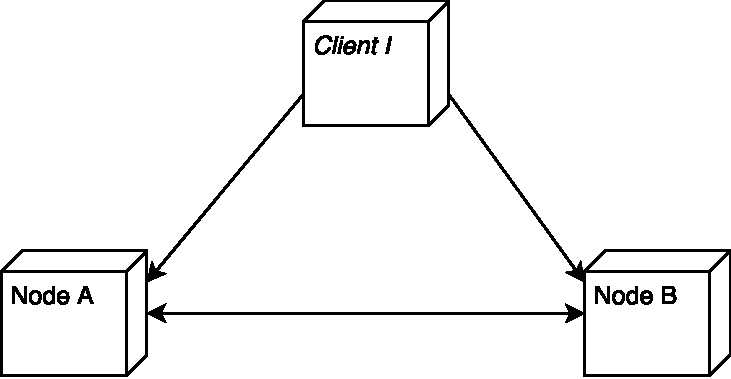
\includegraphics[width=0.5\linewidth]{resources/integration_test_small}
	\caption[Minimal integration test]{Minimal integration test with one client and two nodes.}
	\label{fig:integrationtestsmall}
\end{figure}

\begin{figure}
	\centering
	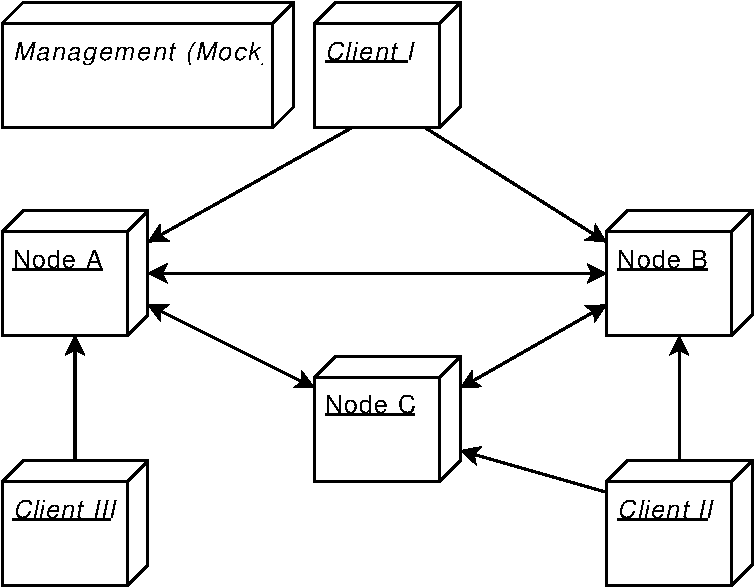
\includegraphics[width=0.5\linewidth]{resources/integration_test_medium}
	\caption[Medium integration test]{Medium integration test with three clients and three nodes.}
	\label{fig:integrationtestmedium}
\end{figure}

These two, rather small network styles will probably be the most commonly used deployments, yet cover most of the possible problems that may occur.

The integration tests are to be run automatically at least on every tagged release (i.e. at least once every sprint).

To write integration tests as effective as possible, we created a testing library written in python that enabled us to write comprehensive black box tests. In this framework, the internals on how to launch and configure clients and nodes is encapsulated in classes. Using this abstraction, we decided to launch clients and nodes in separate docker containers, so that they are as isolated as possible. All containers used in a test case are connected to a dedicated docker network which eliminates possible interferences with other network services.

We wrote integration tests that verify that a backup can be created, is replicated onto other nodes and is restored flawlessly.

Tests for the fault tolerance, e.g. what happens if a node goes down during a backup, could be implemented as integration tests as well.

\subsection{Test coverage}
Tarpaulin does not (yet) cover fn definitions that span over multiple lines and generated code (macros - e.g. error types,  use statements, else branches) 53.5\%. Configuration components lack tests


\subsection{Architecture tests}

Architectural tests are special, manually run tests to verify the scalability of our software architecture.

Our integration testing framework allowed us to write such tests in a simple fashion.

\subsubsection{Size scalability}
As per our requirements in Appendix \ref{requirements}, the architecture should scale up to 100 nodes. To test this scenario, we use the same underlying techniques as in our integration tests (see chapter \ref{integration-tests}), but scale the infrastructure up to the required limits.

Due to the high memory consumption of our prototype, we were not able to conduct this test with a significant amount of data. We conducted one test, in which a file of 5MB was replicated to 99 Nodes which worked just fine.

\subsubsection{Data capacity}
Our requirements (Appendix \ref{requirements}) also state, that a node must be able to handle up to e.g. 2TB of data. To test this requirement, we create large amounts of random data that has to be stored. This is a realistic requirement, as e.g. a compressed image, audio and movie collection might reach such sizes in practice.

Both, the client and the server of the prototype use los of memory during the creation of a backup. It therefore was not possible yet to create a single backup of 2TB. Performing multiple backups in a row of a smaller dataset (i.e. 5 files with a size of 500MB) did not show any sign of a decreasing performance.

\subsubsection{Concurrent Backups}

Times are quite good: 5 concurrent clients that back up onto 3 (randomly chosen) Nodes took
Problematic: All use lots of CPU (for hash creation) and lots of RAM
Further investigation required

Table? (Client, data, target node)

Backup size client1:  12 MB
Backup size client2: 272 MB
Backup size client3: 135 MB
Backup size client4: 384 MB
Backup size client5: 330 MB

Execution time client1: 01.281948s
Execution time client2: 30.701459s
Execution time client3: 17.812313s
Execution time client4: 35.111059s
Execution time client5: 29.004889s